% CoRL 2026 abstract one-pager (for OpenReview abstract phase / sharing).
% Build: make -C paper abstract

\documentclass[10pt]{article}

\usepackage[letterpaper, margin=0.85in]{geometry}
\usepackage[T1]{fontenc}
\usepackage{lmodern}
\usepackage{microtype}
\usepackage{amsmath,amssymb}
\usepackage{graphicx}
\usepackage{booktabs}
\usepackage{enumitem}
\usepackage{hyperref}
\usepackage{xcolor}

\graphicspath{{figures/}}

\newcommand{\AV}{\ensuremath{\mathrm{AV}}}
\newcommand{\AR}{\ensuremath{\mathrm{AR}}}
\newcommand{\hvec}{\mathbf{h}}
\newcommand{\code}[1]{\texttt{\small #1}}

\setlength{\parskip}{0.35em}
\setlength{\parindent}{0pt}
\setlist[itemize]{nosep, leftmargin=*, topsep=2pt, itemsep=1pt}

\pagestyle{empty}

\begin{document}

\begin{center}
  {\LARGE\bfseries When Reconstruction Passes:\\[0.15em]
  Natural-Language Autoencoders on VLA Activations\\
  Fail Grounding and Semantic Steering}\\[0.6em]
  {\normalsize Anonymous Author(s) \textbar\ Anonymous Institution \textbar\ anonymous@domain.com}\\[0.15em]
  {\small\textit{Submitted to the 10th Conference on Robot Learning (CoRL 2026). Do not distribute.}}
\end{center}

\vspace{0.4em}
\noindent\textbf{Abstract.}\quad
Natural-language autoencoders (NLAs) map neural activations to text and back,
offering readable interfaces to model internals.
We port the NLA recipe to the GR00T vision-language-action (VLA) backbone:
extract per-token hidden states, train an activation verbalizer (\AV) and
reconstructor (\AR), and inject \AR{} outputs as live backbone steers in
LIBERO simulation.
Supervision uses a multimodal \emph{teacher} (frames + instruction), not
human descriptions of what \(\hvec\) encodes---a confound inherited from the
original LLM setting.
We release \code{nla-groot} and a three-axis evaluation protocol:
(1)~offline reconstruction and retrieval,
(2)~vision-grounded caption judging,
(3)~closed-loop steer A/B (matched vs.\ mismatched language).
On our main checkpoint, reconstruction metrics pass while grounding,
anti-template specificity, and semantic steering fail; aggregate scores
\textbf{hide} collapse on \code{image\_patch} tokens, where retrieval
margin is near zero.
\textbf{Claim:} NL autoencoders on VLA activations are misleading without
vision-grounded and behavioral checks \emph{stratified by token role}---use
this protocol before trusting captions or steering policies with language.

\vspace{0.25em}
\noindent\textbf{Keywords:} vision-language-action models, interpretability, activation steering, robot learning

\vspace{0.35em}
\noindent\textbf{Contributions.}
\begin{itemize}
  \item \textbf{Port \& tooling:} NLA (\AV{}/\AR{}) on GR00T layer-16 activations with live LIBERO steering hooks and open \code{nla-groot} pipeline.
  \item \textbf{Three-axis scorecard:} pre-registered reconstruction/retrieval, vision-grounded caption judge, and closed-loop steer A/B (\(\Delta_{cw}\)).
  \item \textbf{Negative result:} pooled metrics pass while \code{image\_patch} retrieval margin is near chance (0.003), anti-template judge fails (8.3\%), and \(\Delta_{cw}=0\)---aggregate PASS hides vision-slot collapse.
\end{itemize}

\vspace{0.2em}
\begin{minipage}[t]{0.48\textwidth}
  \centering
  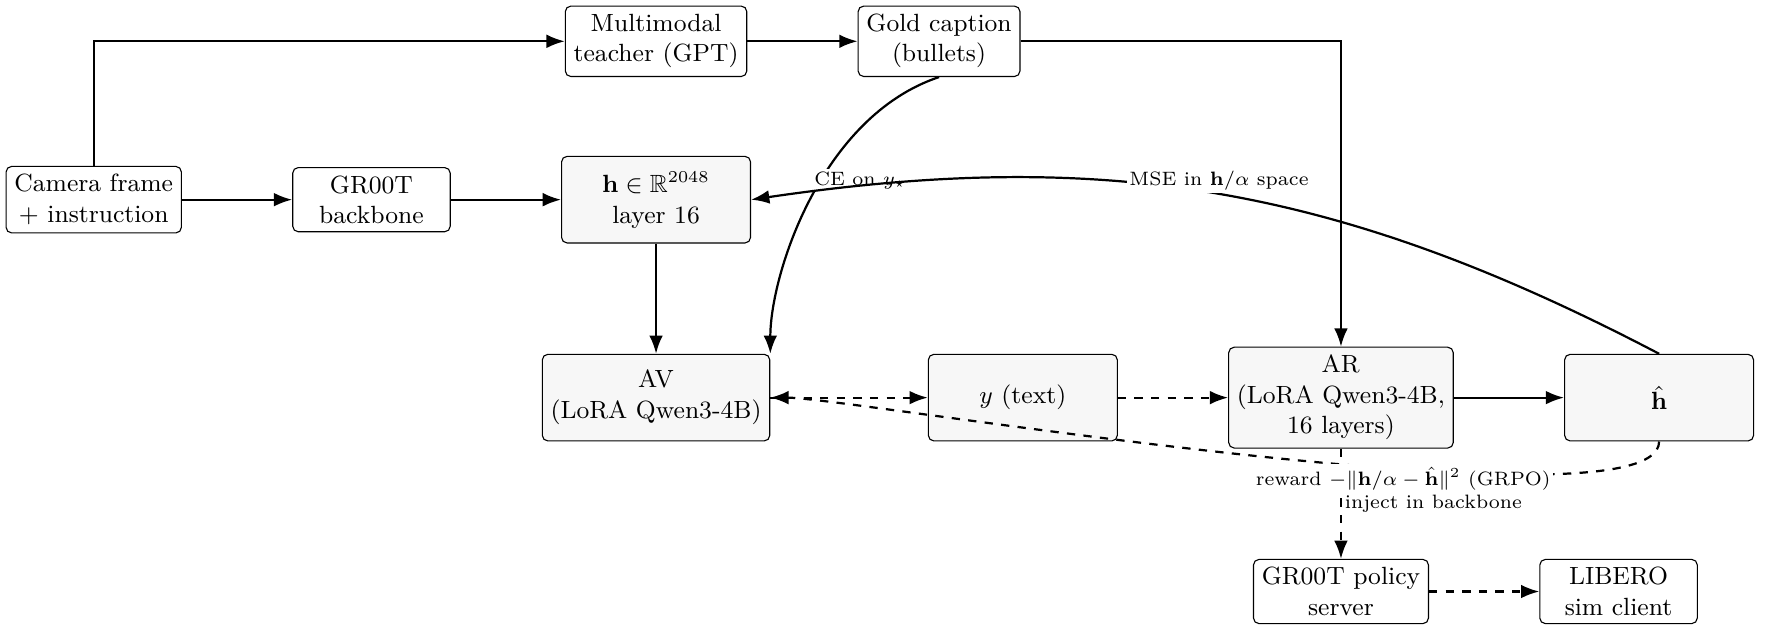
\includegraphics[width=\linewidth]{system_overview.png}\\[-0.2em]
  {\small\textbf{Figure 1.} Training (solid) and inference steering (dashed).}
\end{minipage}\hfill
\begin{minipage}[t]{0.48\textwidth}
  \centering
  {\small\textbf{Table 1.} Headline V3 scorecard (\code{libero\_4suite\_v3}).}\\[0.3em]
  \small
  \begin{tabular}{@{}lrrl@{}}
    \toprule
    Metric & Value & Thr. & \\
    \midrule
    retrieval\_margin & 0.124 & 0.05 & PASS \\
    judge\_anti\_template & 0.083 & 0.50 & FAIL \\
    sim\_correct\_minus\_wrong & 0.000 & 0.05 & WARN \\
    \midrule
    \code{image\_patch} margin & 0.003 & --- & near chance \\
    \bottomrule
  \end{tabular}
\end{minipage}

\vspace{0.35em}
\noindent\textbf{Takeaway.} Reconstruction certifies a text--vector codec, not pixel grounding or semantic steering.
Stratify evaluation by token role (\code{image\_patch} vs.\ \code{last\_text}) before deploying NL interfaces on VLAs.
Code and scorecard scripts: anonymous repository (placeholder URL for review).

\end{document}
